\documentclass[10pt]{beamer}
\usetheme{Antibes}

\tolerance 99999
\hbadness 99999

\usepackage{amsmath,amsthm,amssymb,color,latexsym}
\usepackage{cancel}
\usepackage{graphicx}
\setbeamertemplate{items}[ball]


\newenvironment{points}{\vspace{0.3cm} \begin{enumerate}[label={(\alph*)}]}{\end{enumerate} \vspace{0.2cm}}

\title[Introduction to Cosmology - Ryden] %optional
{Presentation for \textbf{Introduction to Cosmology} \\ \textit{- Barbara Ryden}}

\author[Abhiram Tilak] % (optional, for multiple authors)
{\textbf{Abhiram Tilak}}

\institute[IIITH] % (optional)
{
	\textit{	\tiny{CND Dual Degree}} \\
	\textit{IIIT Hyderabad}
}


\date[16th July 2024] % (optional)
{16th July 2024}


\AtBeginSection[]{
  \begin{frame}
  \vfill
  \centering
  \begin{beamercolorbox}[sep=8pt,center,shadow=false,rounded=true]{title}
    \usebeamerfont{title}\huge \insertsectionhead\par%
  \end{beamercolorbox}
  \vfill
  \end{frame}
}

\begin{document}

\begin{frame}
	\titlepage
\end{frame}

\begin{frame}
\frametitle{Table of Contents}
\tableofcontents
    \end{frame}


% 1 - Introduction

\small
\section{Introduction}
\begin{frame}{Introduction}
	Cosmology is the study of dynamics of Universe.

	\textbf{Units:}
	\begin{itemize}[<+->]
	\item
	The units of measurement in cosmological scales are

\item \textbf{Distance:} \begin{itemize}

	\small
\item $$ 1 AU = 1.50 \times 10^{11} m  $$
	\centering
	( Distance between earth and Sun )
\item $$ 1 pc = 3.09 \times 10^{16} m  $$
	\centering
	( Distance at which 1 arcsecond subtents 1 AU )

	\centering
	A common metric is Mpc ( Mega $10^6$ parsecs )
\end{itemize}
    \end{itemize}
\end{frame}

\begin{frame}{Introduction}{Units}

    \begin{itemize}[<+->]
\item \textbf{Mass:} \begin{itemize}

	\small
\item $$ 1 M_* = 1.99 \times 10^{30} kg  $$
	\centering
	( Mass of Sun (average star) )

\end{itemize}

\item  \textbf{Luminosity: } \begin{itemize}
		\item $$ 1 L_* = 3.83 \times 10^{26} Watts $$
	\centering
			(Luminosity of sun)
	\end{itemize}

\item \textbf{Time:}
 \begin{itemize}[<+->]
		\item $$ 1 yr = 3.16 \times 10^{7} seconds $$
			(One Year on Earth ) A common metric is Gyr ($10^9$
			years)
	\end{itemize}


    \end{itemize}
\end{frame}


\begin{frame}{Introduction}{Units}

    \begin{itemize}[<+->]
\item \textbf{Energy:} \begin{itemize}

	\small
\item
	\centering
	$$ 1 eV = 1.6 \times 10^{-19} J $$
	( Columb Energy of a charged electron ) A common measure
	is MeV used to get rest energy ($10^6$ eV)

\end{itemize}
    \end{itemize}
\end{frame}



\begin{frame}{Introduction}{Plank's Units}

	Based on universal constants like $G, c, \hbar$, which remain
	constant throughout the universe

	\begin{itemize}[<+->]
		\item $$ l_p = \sqrt{\frac{G\hbar}{c^3}} = 1.62 \times 10^{-35}
			m$$
		\item $$ M_p = \sqrt{\frac{\hbar c}{G}} = 2.18 \times 10^{-8} kg $$
		\item $$ t_p = \sqrt{\frac{G\hbar }{c^5}} = 5.39 \times 10^{-44}
			s$$
		\item $$ E_p = M_p c^2 = 1.96 \times 10^{9} J $$
	\end{itemize}
\end{frame}

\section{Fundamental Observations}

\begin{frame}{Fundamental Observations}{Sky is Dark}
	Heinrich Olber came up with the observation that
	the Sky is dark, when it really shouldn't be. If we assume universe
	to be infinitely long, and indefinitely long, then using calculated
	parameters like $n$ (number density of stars), $L_*$ luminosity of
	an average star, Radius of star $R_*$, etc, we can see that luminosity of night sky far outweighs the
	luminosity of night sky by 10 trillion.

	Start with the fact that we need only one start with $R_*$ to block
	our view to the rest of the stars behind it. Say this star is at
	distance $\lambda$
	$$ 1 = n V $$
	$$ 1 = n \pi r^2 \lambda $$
\end{frame}

\begin{frame}{Fundamental Observations}{Sky is Dark}
This is called Olber's paradox and there are various explanations to this
effect:
\begin{itemize}[<+->]
	\item \textbf{The space is not transparent and there are particles that absorb
		light.} This can't be true because any body that absorbs light
		will eventually start emitting light like BBR.
	\item \textbf{Assumption that Universe is infinitely large is wrong.}
	\item \textbf{Assumption that Universe has existed forever is wrong.}:
		This supports to a big bang model, rather than a steady state one.
	\item \textbf{If universe were to be constantly expand, then the
		brightness of the light source would decrease as it reaches us.}
		This doesn't explain why we don't see stars in all directions
		though.
\end{itemize}
\end{frame}


\begin{frame}{Fundamental Observations}{Universe is Isotropic and Homogenous}

In small scales its not. In the orders of 100 Mpc though we can consider
universe to be both "Isotropic" and "Homogenous"


\includegraphics[width=4in]{1}

\end{frame}

\begin{frame}{Fundamental Observations}{Early Observations}
    Early astronomers and philosophers like Galileo and Coppernicus disproved the
    geocentric model and adopted the heliocentric one. But according to
    Coppernicus, even the heliocentric model doesn't explain the speciality of
    our place.

    This leads us to the Coppernican principle that when built on top of it
    leads us to the Cosmological principle.

    "There is nothing special or privileged about our location in the
    universe." - Coppernicus

    "We're not only not number one, but we are next to none" - Cosmological
    Principle.
\end{frame}


\begin{frame}{Fundamental Observations}{Redshift is proportial to Distance}

Redshift is caused due to Doppler's effect in EM waves which cause a shift in
the emitted wavelength versus the observed
$$ \frac{v}{c} \approx z = \frac{\lambda_{ob} - \lambda_{em}}{\lambda_{em}} $$
We can use the doppler shift to explain that, objects which move farther away
produce a red shift and the ones, coming closer cause blue shift.

Scientists like Lemaitre, observed that 37 of 42 observed objects were
redshifted rather than blueshifted. Hubble was another scientists who calculated
that there is a linear relation between the redshifts (z) and the distances of
the objects from Earth.

$$ z = \frac{H_0}{c} r $$

Using $ \frac{v}{c} \approx z $, we get
$$ v = H_0r  $$


\end{frame}

\begin{frame}
 Does this mean that all particles are moving
away from us? That would violate the cosmological principle.

\begin{columns}
	\column{.5\textwidth}
	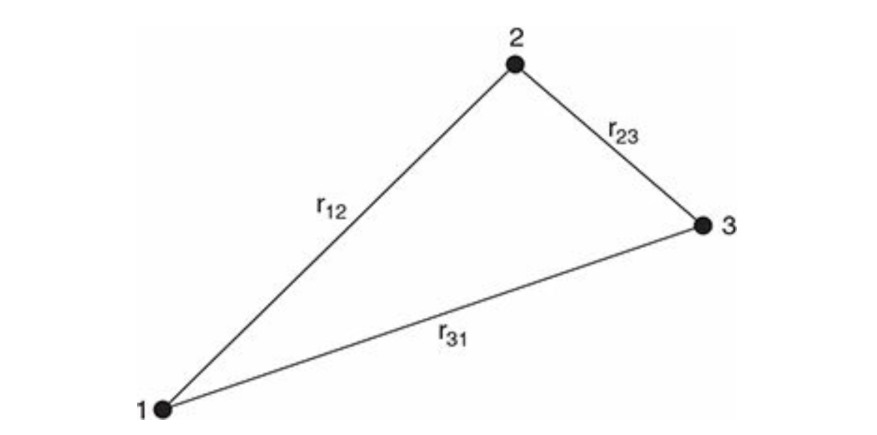
\includegraphics[width=\textwidth]{2}
	\column{.5\textwidth}
	$$ r_{12} = a(t)r_{12}(t_0) $$
	$$ v_{12} = \frac{dr_{12}}{dt} = \dot a(t)r_{12}(t_0) = \frac{\dot a}{a}
	r_{12}(t)$$
	Thus,
	$$ \frac{v_{12}(t)}{r_{12}(t)} = \frac{\dot a}{ a } = H_0 $$

\end{columns}

\vspace{1cm}

This means the universe has expanded in linear fashion. Thus we can
estimate the lifetime of universe by $t = \frac{r}{v} = H_0^{-1}$ of any object.
This is a good estimated of the lifetime of universe, $t_0 = 14.38 Gyr$.

\end{frame}

\begin{frame}{Fundamental Observations}{Different Types of Particles}
    I will cover only photon and neutrino.

    \begin{itemize}[<+->]
	    \item \textbf{Neutrino:}
		    This is mostly a relativistic particle but has rest mass
		    energy of about $10^{-2} eV$. There are three types of
		    neutrinos, and each of these type have three mass states
		    $(m_1, m_2, m_3)$. Due to quantum occilations the rest
		    energy keeps changing and this  energy can be calculated.
		    $$ (m_2^2 - m_1^2)c^4 \approx 7.5 \times 10^{-5} $$
		    $$ (m_3^2 - m_2^2)c^4 \approx 2.4 \times 10^{-3} $$
	    But this doesn't give us an estimate of individual mass states.
	    Approximations can be made by calculating  the rest energy of
	    sum of $(m_e + m_t + m_u) = (m_1 + m_2 + m_3)$, which comes out to
	    be between $(0.057, 0.3) eV$.
    \end{itemize}
    $$  $$

\end{frame}

\begin{frame}
	\begin{itemize}[<+->]
	    \item \textbf{Photon:}
		    Even though they have no mass, they do have energy density
		    which can be calculated using the blackbody function:
		    $$ \epsilon(f)df = \frac{8\pi h}{c^3} \frac{f^3 df}{
		    e^{\frac{hf}{kT}} - 1 } $$

		    We can use it to calculate the energy and the number density
		    by integrating over all frequencies.
		    $$ \epsilon_\gamma = \alpha T^4 $$
		    Where $\alpha = \frac{\pi^2}{15} \frac{k^4}{\hbar^3 c^3}$,
		    $$ n_\gamma = \beta T^3 $$
		    Where $\beta = \frac{2.4041}{\pi^2} \frac{k^3}{\hbar^3 c^3}$,

		    One great thing about radiation is that we can calculate the
		    temperature corresponding to a give frequency using
		    $$ E_{mean} = h f_{mean} = 2.7 k T  $$
		  \end{itemize}
\end{frame}

\begin{frame}{Fundamental Observations}{Comsological Microwave Background}
There have been other models being proposed too which go against the fact that
universe is expanding linearly, one such is Steady State model.
$$ \frac{dr}{dt} = H_0 r $$
$$ r = e^{H_0 t}$$
Another postulate of this model is that the Mass density of the universe is
constant. But if universe is expanding and density is constant, that would mean
new matter is being produced, but that violates various laws of physics.

But this model got disproved once the CMB waves were discovered and it gave an
accurate representation


\end{frame}

\begin{frame}
	It was observed that there is an isotropic background of microvawe
	radiation all over the universe and the wavelength of this corresponds to
	that of microwaves, thus temperature can be calculated by above relation
	as $T_0 = 2.7255 K$. This can be again used to calculate the energy
	density and the number density as.
	$$ \epsilon_\gamma = 4.175 \times 10^{-14} MeV/m^3
	, n_\gamma = 4.107 \times 10^8 m^{-3} $$

	It is said that CMB is a relic to the past when the radiation was so
	dominant, that it used to render the universe opaque and matter was
	ionized. Then this energy density fell off to a point where the energy
	of these photons couldn't photoionize matter anymore.

	We can start with the second law of thermodynamics and actually
	calculate the dependence of temperature of CMB to the expansion
	coefficient
	$$ dQ = dE + PdV $$
\end{frame}

\section{Newton Vs. Einstein}

\begin{frame}{Newton Vs. Einstein}{Newton's Laws}
	According to newton's laws we know that
	$$ F = m_i a $$
	where $m_i$ is inertial mass.

	Newton also proposed the Gravitational Law:
	$$ F =- \frac{GM_g m_g}{r^2} $$

	Equivalence law states that the property that determines, how strongly
	an object is pulled by gravity, also tells us how it accelerates by ANY
	force. Proof is simple observations made by Galileo on objects on earth.

	Using Guass's law and other vector algebra we can define a quantity that
	measures how much Gravity acts on a given point in space using
	\textbf{Poisson's Law}:
	$$ \nabla^2 \Phi = 4\pi G \rho $$
\end{frame}

\begin{frame}
	This quantity is called the Gravitational potential $\Phi$, and is
	divergence of the acceleration due to gravity of a test mass,
	$$ \vec a = - \vec \nabla \cdot \vec \Phi $$

	This Poission's equation basically relates Gravity with mass density.
\end{frame}


\begin{frame}{Newton Vs. Einstein}{Special Theory of Relativity}
	Postulates:
	\begin{itemize}[<+->]
		\item In all intertial frames (where laws of physics are valid),
			the basic laws of physics are same.
		\item If above is true, then for all the frames Maxwell's laws
			are true and we calculate the speed of light to be c.
        \end{itemize}

	This means say in two different frames, the displacement of light in both
	of these frames must be equal.
	$$ c^2t^2 = x^2 + y^2 + z^2 $$
	$$ c^2t'^2 = x'^2 + y'^2 + z'^2 $$

	Thus we have to use the lorentz tranformation instead:
	$$ x' = \gamma(x - vt), t' = \gamma(t - vx/c^2), y'=y, z'=z $$
	Where $\gamma = (1 - v^2/c^2)^{-1/2}$

\end{frame}

\begin{frame}
	So here, we need to find a quantity that is constant accross these
	intertial frames. This quantity is called spacetime (minkowski metric)

	$$ ds^2 = ct^2 - dx^2 - dy^2 - dz^2 $$
	or simply
	$$ ds^2 = ct^2 - dl^2 $$

	Light is said to travel a null geodesic path, which is in accordance
	with the fermat's principle that, light always takes the path with
	shortest time (now spacetime). Thus $ds^2 = 0$
\end{frame}


\begin{frame}{Newton Vs. Einstein}{General Theory of Relativity}
	The above calculations are considering that there is no curvature in
	space and there is no gravity acting.

	Einstein used the
	Equivalence principle to explain that light must bend due to gravity
	even though it has no mass.

	Thus Einstein concludes that it is not mass that makes things bend but
	the Energy. Mass and energy for non-relativistic objects are
	interconvertible using the $E = mc^2$, and Energy is interconvertible
	with momentum for relativistic objects as $E = pc$
\end{frame}


\begin{frame}{Newton Vs. Einstein}{Defining Curvature}
	There are two types of uniform curvatures, postive and negetive (taking
	2-D for example):
	\begin{itemize}
		\item  Uniform Positive Curvature:
			$$ \alpha + \beta + \gamma = \pi + A/R_0^2  $$
			When we measure a distance $dl$ along this curved
			surface, then interms of spherical coordinates it can be
			written as:
			$$ dl^2 = dr^2 + R^2 sin^2(r/R)d\theta^2 $$
		\item  Uniform Negetive Curvature:
			$$ \alpha + \beta + \gamma = \pi - A/R_0^2  $$
			When we measure in spherical coordinates, the value
			comes out to be
			$$ dl^2 = dr^2 + R^2 sinh^2(r/R)d\theta^2 $$

        \end{itemize}
\end{frame}

\begin{frame}{Newton Vs. Einstein}{Defining Curvature}
	When we try to scale this to 3-D we get:

	Flat:
	Uniform positive curvature gives:
	$$ dl^2 = dr^2 + r  [d\theta^2 + sin^2 \theta d\phi^2]$$
	Uniform positive curvature gives:
	$$ dl^2 = dr^2 + R^2 sin^2(r/R)  [d\theta^2 + sin^2 \theta d\phi^2]$$
	Negetive positive curvature gives:
	$$ dl^2 = dr^2 + R^2 sinh^2(r/R)  [d\theta^2 + sin^2 \theta d\phi^2]$$

	We can generalize this by substituiting variables like $S_k(r)$ and
	$d\Omega$. Where
	$$ d\Omega = d\theta^2 + sin^2\theta d\phi^2 $$
\end{frame}

\begin{frame}
	$$ S_k(r) = \begin{cases}
		Rsin(r/R) & (\kappa = 1) \\
		r & (\kappa = 0) \\
		Rsinh(r/R) & (\kappa = -1) \\
	\end{cases}$$
	Which makes the distance equation as:
	$$ dl^2 = dr^2 + S_k(r)^2 d\Omega^2 $$

\end{frame}

\begin{frame}{Newton Vs. Einstein}{Robertson-Walked Metric}
	This metric is a curved generalization to the Minkowski metric given by
	$$ ds^2 = -c^2 dt^2 + a(t)^2 [ dr^2 + S_k(r)^2 d\Omega^2 ] $$

	This is important because it takes into account that, the expansion
	coefficient determines how the universe moves.
\end{frame}


\begin{frame}{Newton Vs. Einstein}{Proper Distance}
	When we measure distance in a curved / expanding universe we don't take
	into account the error which is caused because of the expansion
	coefficient. Proper distance does.
	$$ ds^2  = a(t)^2 [dr^2 + S_\kappa (r)^2 d\Omega^2] $$
	Taking angular component to be zero if we observe object directly.
	$$ ds = a(t)dr $$
	$$ d_p(t) = a(t)r $$

	If you observe this proves hubble's law:
	$$ v_p(t_0) = H_0 d_p(t_0) $$
\end{frame}

\begin{frame}{Newton Vs. Einstein}{Expansion and red Shift}

	We can use the fact that photons follow geodesic. In the
	robertson-walker equation we have:
	$$ 0 = -cdt^2 + a(t)^2 (dr)^2 $$
	$$ a(t).dr = c.dt $$
	$$ \int^{t_o}_{t_e}\frac{dt}{a(t)} = \int^{r}_{0} dr = r $$
	Integrating between time of observation and emission.

	If we were to calculate for the next crest of the wave we will still get
	r.
	Thus by subtracting we get.
	$$ \int_{t_e}^{t_o} \frac{dt}{a(t)} = \int_{t_e + \lambda_e / c}^{ t_o + \lambda_o / c } \frac{dt}{a(t)} $$
	$$ \int^{t_e + \lambda_e / c}_{t_e} \frac{dt}{a(t)} = \int^{ t_o +
	\lambda_o / c }_{t_o} \frac{dt}{a(t)} $$
\end{frame}

\begin{frame}
	Using the fact that expansion of universe barely happens when the crest
	propogates we use:
	$$ \frac{\lambda_e}{a(t_e)} =  \frac{\lambda_o}{a(t_o)}$$
	$$ 1 + z =  \frac{1}{a(t_e)} $$
\end{frame}

\section{Cosmic Dynamics}

\begin{frame}{Cosmic Dynamic}{Einstien's Field Equation}
	$$ G_{\mu \nu} = \frac{8\pi G}{c^4} T_{\mu \nu} $$
	The $G$ term is called Einstein's metric tensor (describes the curvature
	of universe at all x,y,z,t) and the T term is called
	the stress-energy metric tensor.
\end{frame}

\begin{frame}{Cosmic Dynamic}{Friedmann's equation}
	An equation that links the Expansion of universe, Curvature and the
	Mass-energy was required including terms $a(t), R_0, \kappa,
	\epsilon(t)$.


	$$ \left( \frac{\dot a}{a} \right)^2 = \frac{8\pi G}{3c^2}\epsilon(t) -
	\frac{\kappa c^2}{R_0^2} \frac{1}{a(t)^2}$$

	Friedmann proved this for General theory of relativity, but we will
	prove it using the Newtonian Way.

	To get to this, start with this take, a sphere that is contracting
	because of its own action of gravity. Acceleration can be given as
	$$ \frac{d^2R_s(t)}{dt^2} = - \frac{GM_s}{R(t)^2} $$


\end{frame}

\begin{frame}{Cosmic Dynamic}{Critical Density}
	We can calculate the energy density using above relation for a good
	estimate case senario where $\kappa = 0$, and $H(t) = \frac{\dot a}{a}$
	is the hubble parameter. We get

	$$ \epsilon_c(t) = \frac{3c^2}{8\pi G} H(t)^2  $$
	For the current time, we can substituite the Hubble's constant and get
	$\epsilon_{c,0} = 4870 MeV/m^3$ which also gives us mass density if you
	divide by $c^2$.

	We define Density parameter to be that of ratio with the critical
	density for any universe as:
	$$ \Omega (t)  = \frac{\epsilon(t)}{\epsilon_c(t)} = 1 + \frac{\kappa
	c^2}{R_0^2 a(t)^2 H(t)^2} $$

	Using we get the relation to finally get rid of $\kappa$:
	$$ \frac{\kappa}{R_0^2} = \frac{H_0^2}{c^2} (\Omega_0 - 1) $$
\end{frame}


\begin{frame}{Cosmic Dynamic}{Fluid Equation and Acceleration Equation}
	We know that Friedmann equation in the end of the day comes from energy
	conservation, so we can use the first law of  thermodynamics to get a
	similar equation.

	We start with
	$$ \dot E + P \dot V = 0 $$
	and finally get:
	$$ \dot \epsilon + 3 \frac{\dot a}{a} (\epsilon + P) = 0 $$

	We can use this in the friedmann equation to get the acceleration
	equation.
	$$ \frac{\ddot a}{a} = \frac{4\pi G}{3c^2}\left( \epsilon + 3P \right) $$
\end{frame}

\begin{frame}{Cosmic Dynamic}{Equations of State}
	We need another set of equations to solve the friedmann equation:
	This equation called called equation of state is a relation between the
	pressure used in fluid equation and energy density
	$$ P = w \epsilon  $$

	This w can vary with the substance used. For $w = 0$ for matter (can be
	solved by using ideal gas equation) and for radiation the $w = 1/3$
	comes from statistical mechanics and boson nature.
\end{frame}


\begin{frame}{Cosmic Dynamic}{Cosmological constant}

	Einstein first introduced this to explain the static nature of universe
	but cosmologists now use it because the default calculation of hubble's
	constant are very underestimated. When added to the friedmann equation,
	the cosmological constant looks like
	$$ \left( \frac{\dot a}{a} \right)^2 = \frac{8\pi G}{3c^2}\epsilon(t) -
	\frac{\kappa c^2}{R_0^2} \frac{1}{a(t)^2} + \frac{\Lambda}{3}$$

	Its as if cosmological constant had its own energy density which doesn't
	very with time or expansion.
	$$ \left( \frac{\dot a}{a} \right)^2 = \frac{8\pi G}{3c^2}(\epsilon(t) +
	\epsilon_\Lambda )-
	\frac{\kappa c^2}{R_0^2} \frac{1}{a(t)^2}$$

	If we were to call, $\epsilon_k = \epsilon + \epsilon_\Lambda$, that
	would mean to keep the fluid equation constant we need. $w = -1$, which
	means there is an attrative force.



\end{frame}

\begin{frame}

	This is same as what Einstein did to add $\Lambda$ to the Newton's
	equation. (acceleration equation, when einstein's universe is static)
	$$ 0 = - \frac{4\pi G}{3} + \frac{\Lambda}{3} $$
	When we solve for friedmann equation too (with static universe) we get.
	$$ R_0 = \frac{c}{\Lambda^{1/2}} $$
\end{frame}

\section{Model Universes}

\begin{frame}{Model Universes}{Evolution of energy density}

	$$ P = w\epsilon; \hspace{1em} \dot\epsilon + 3\frac{\dot
	a}{a}(\epsilon + P) = 0 $$

By solving the state equation and the fluid equation alone, we can come up
with a relation
$$ \epsilon_i (a) = \epsilon_{i,0} a^{-3(1+w_i)}$$

The can be multiple explanations for why energy density decreases
\begin{itemize}[<+->]
	\item For matter, we have a $\epsilon \propto a^{-3}$, taking the value of
		$E_{mean}$ to be rest mass energy and constant we have that, the
		number density decreases cubically
	\item For radiation,$\epsilon \propto a^{-3}$ is due to the wavelength
		begin expanded (Emean reduces), but same the number density
		decreases.
	\item For Lambda matter, we have no dependence that means energy remains
		constant
\end{itemize}
\end{frame}


\begin{frame}{Model Universes}{Solved Friedmann equation}
Now if we use the relation we got by solving equation of state and fluid
equation in the friedmann equation we get:

$$ \dot a^2 = \frac{8\pi G}{3c^2} \sum \epsilon_i a^{-(1+3w_i)} -
\frac{\kappa c^2}{R_0} $$

Assuming the universe contains, Curvature, Matter, Radiation and Comsmological
Constant.

$$  \dot a^2 = \frac{8\pi G}{3c^2} ( \epsilon_\Lambda + \frac{\epsilon_r}{a^4} +  \frac{\epsilon_m}{a^3} ) -
\frac{\kappa c^2}{R_0}  $$

Using the relation in 4th chapter about curvature and using the definition of
$\epsilon_{c,0} = \frac{3c^2}{8\pi G}H_0^2 $ and $\frac{\kappa c^2}{R_0^2} = H_0^2(\Omega_0 - 1)$

$$ \frac{H^2}{H_0^2} = \frac{\Omega_{r,0}}{a^4} +
	\frac{\Omega_{m,0}}{a^3} + \Omega_{\Lambda,0} + \frac{1 - \Omega_{0}}{a^2} $$


\end{frame}

\begin{frame}{Model Universes}{General Procedure to solve the Model Universe}

\begin{itemize}[<+->]
	\item Using the friedman equation find out a relation between a(t) and
		t.
	\item Calculate z now using this relation.
	\item Calculate $d_p(t_o)$ interms of to and te. Use te = 0 to get
		horizon distance if exists.
	\item The get the $d_p(t_o)$ in terms of z instead of time.
	\item finally divide by 1+z to calculate $d_p(t_e)$.
\end{itemize}

The first part is usually the hardest part for more complex universes, but it
is simple for, empty universe (direct proportion), single flat component universe
(compare powers on the RHS and LHS).

by comparing powers we get:
$$ a(t) = \left(\frac{t}{t_0}\right)^{2/3+3w} $$

\end{frame}

\begin{frame}{Model Universes}{Empty Universes}
	When universe is empty (no energy density) the friedmann equation can be
	written as:
$$ \dot a^2 = - \kappa c^2 / R_0^2 $$

Values $\kappa = -1$, gives an interesting case where universe is expanding
linearly.

$$ \dot a^2 =  c^2 / R_0^2 $$
$$ a = \pm ct/R_0 $$

Finding $\frac{\dot a}{a} = H_0 = 1 / t_0$, which is original estimation of
hubble's constant that hubble performed.

The horizon distance is infinite and the proper distance in-terms of redshift comes out to be:
$$ d_p(t_0) = ct_0 \int^{t_o}_{t_e} \frac{dt}{a(t)} = \frac{c}{H_0} ln (1+z)$$

\end{frame}


\begin{frame}{Model Universes}{Single component}

A single component universe the friedmann equation can be written as:
$$ \dot a^2 = \frac{8\pi G\epsilon_0}{3c^2} a^{-(1+3w)} $$

Thus solving for relation between a and t.
$$ a(t) = \left( \frac{t}{t_0} \right)^{2/(3+3w)} $$

Using above relations we get some good usable relations like:
$$ d_p (t_0) = \frac{c}{H_0} \frac{2}{1+3w} [ 1 - (1+z)^{-(1+3w)/2} ] $$
$$ d_{Hor} (t_0) = \frac{c}{H_0} \frac{2}{1+3w} $$

\end{frame}


\begin{frame}{Model Universes}{Single component}

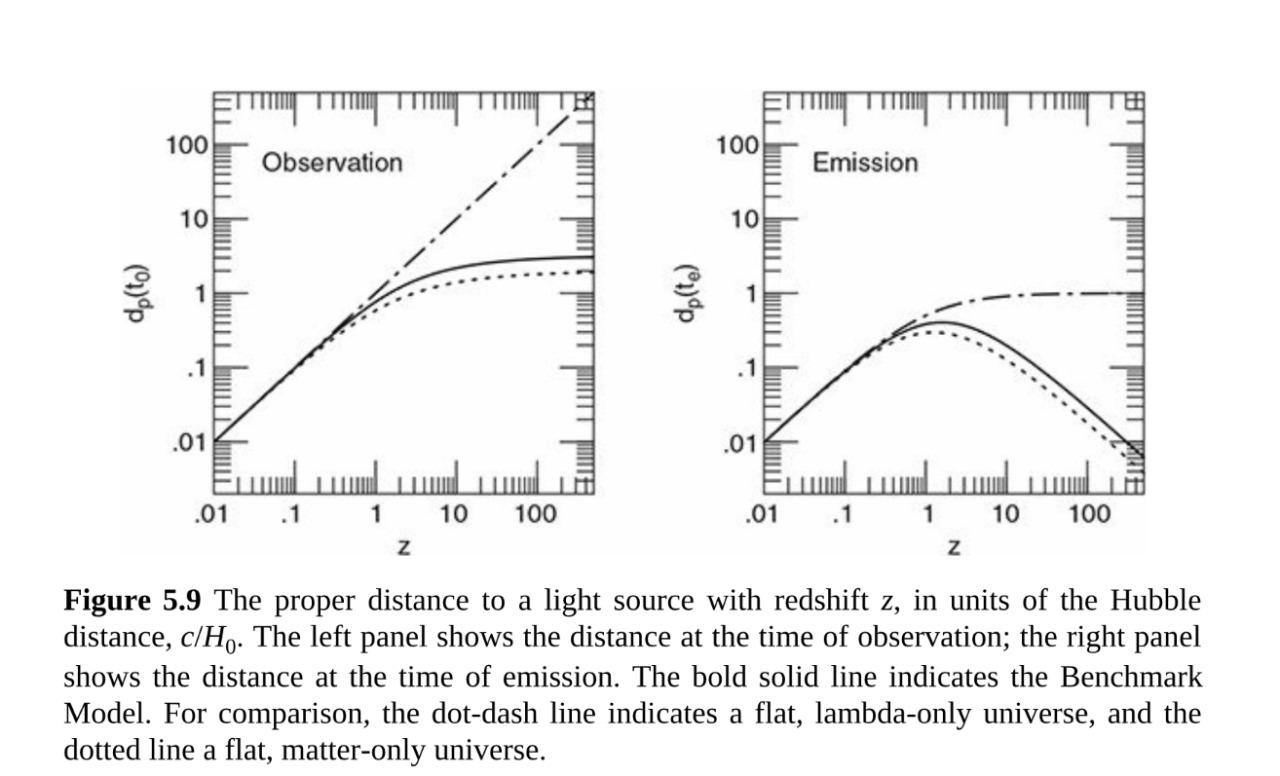
\includegraphics[width=2.2in]{3}
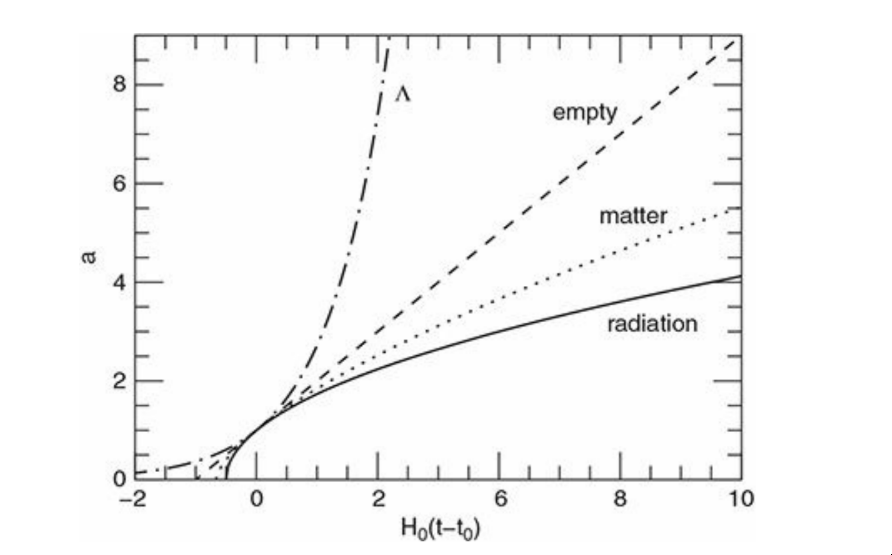
\includegraphics[width=2in]{6}

\end{frame}

\begin{frame}{Model Universes}{Multi component}

	It becomes difficult to integrate and find exact relations in multi
	component universe, hence most of the analysis is done frome the reduced
	version of friedmann equation itself.

	$$ \frac{H^2}{H_0^2} = \underbrace{\frac{\Omega_{r,0}}{a^4}}_{Radiation} +
	\underbrace{\frac{\Omega_{m,0}}{a^3}}_{Matter}
	+ \underbrace{\Omega_{\Lambda,0}}_{Cosmological constant} +
	\underbrace{\frac{1 - \Omega_{0}}{a^2}}_{Curvature} $$

	Where $\Omega_0 = \Omega_{r,0} + \Omega_{m,0} + \Omega_{\Lambda,0}$;
	and $\Omega_0 = 1 $ only if flat universe is   assumed

	If we vary the density parameters the values, we keep observing
	different dynamics in the universe
\end{frame}

\begin{frame}
	Example (matter + lambda + curvature):
	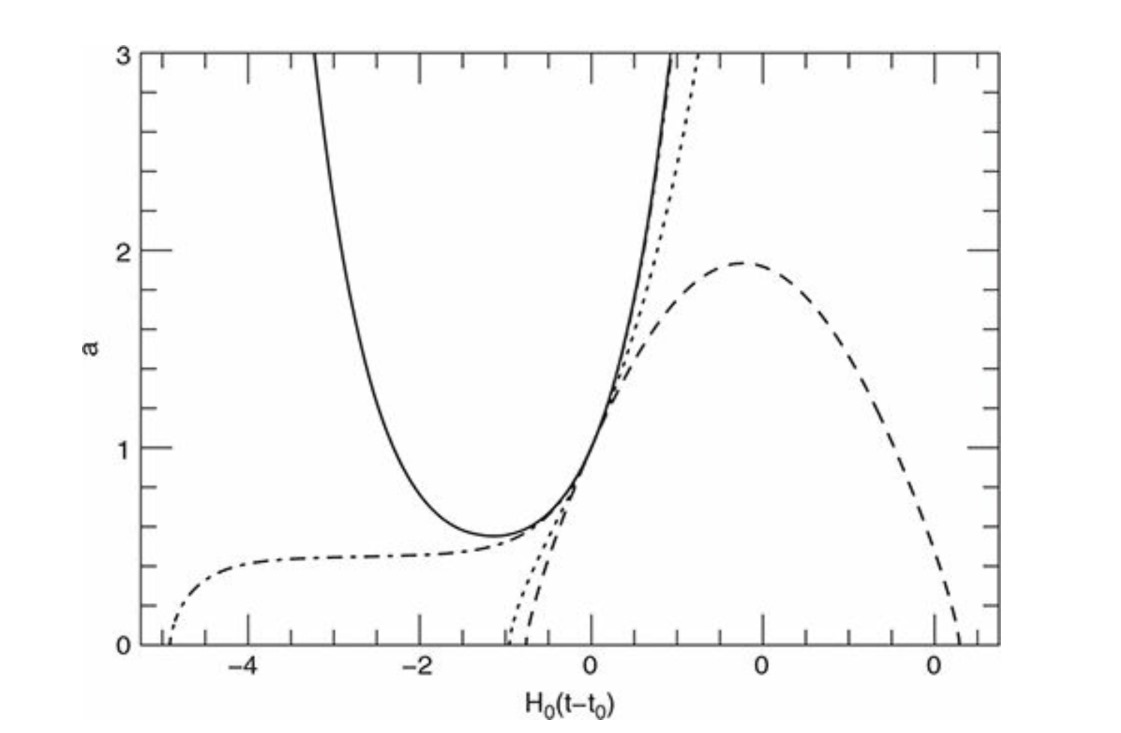
\includegraphics[width=\textwidth]{4}
\end{frame}

\begin{frame}{Model Universes}{Benchmark Universes}

	This is a good estimation to our current universe with the following
	parameters.

	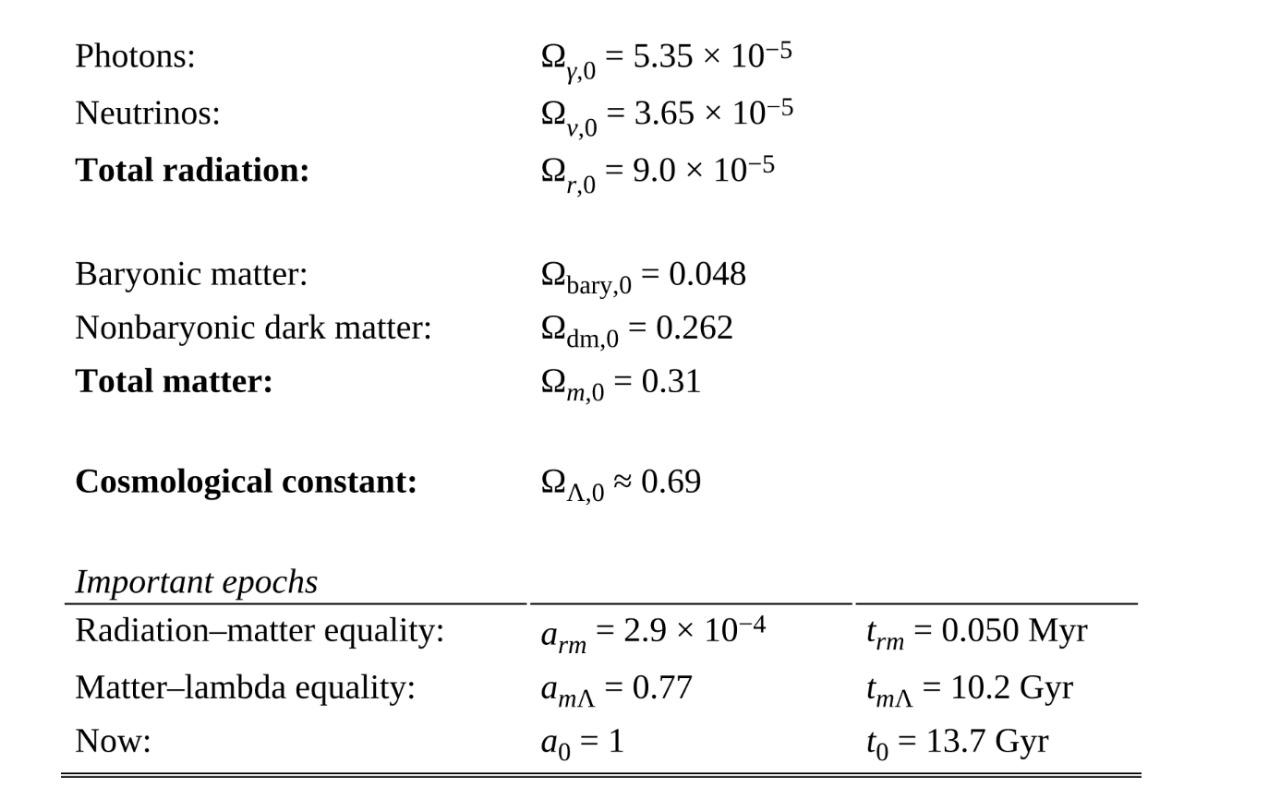
\includegraphics[width=0.9\textwidth]{5}
\end{frame}

\section{Measuring the Cosmological Parameters}

\begin{frame}{Measuring the Cosmological Parameters}{Taylor Expansion of expansion
coefficient}

If we taylor expand a(t) and consider only 2 degree terms

$$ a(t) = a(t_0) + \dot a (t-t_0) + \frac{1}{2} \ddot a (t-t_0)^2 $$

We can define some constants like $H_0 = \frac{\dot a}{a}$, $q_0 = -\frac{\ddot
a}{aH_0^2} = \frac{1}{2} \sum_i \Omega_i (1 + 3w_i)$ (from the acceleration eq).

$$ a(t) = 1 + H_0 (t-t_0) + \frac{1}{2} q_0 H_0^2 (t-t_0)^2 $$

similarly inverse of this can be estimated as:

$$ a(t)^{-1} = 1 - H_0 (t - t_0) + (1 + q_0 /2 ) H_0^2 (t-t_0)^2 $$

This second value is good because we can now calculate the proper distance


\end{frame}

\begin{frame}
	Proper distance in terms of the lookback time $(t_0 - t_e)$ is:
	$$ d_p(t_0) = c \int_{t_e}^{t_o} \frac{dt}{a(t)} = c \int_{t_e}^{t_o}
	(1 - H_0 (t - t_0) + (1 + q_0 /2 ) H_0^2 (t-t_0)^2 ).dt $$
	The $t=t_0$ term cancels out, and only taking upto 2nd degree terms we
	get.
	$$ d_p(t_0) \approx c(t_o - t_e) + cH_0 / 2 (t_0 - t_e)^2 $$

	But the lookback time, is not a good metric that can be easily measured.
	Thus we need to find a way to relate lookback time to redshift.
\end{frame}


\begin{frame}{Measuring the Cosmological Parameters}{Proper Distance}

	If we put $t=t_e$ in the equation.
$$ a(t_e)^{-1} = 1 - H_0 (t_e - t_0) + (1 + q_0 /2 ) H_0^2 (t_e-t_0)^2 $$

And then use the equation $\frac{a(t_0)}{a(t_e)} = 1 + z$, we get
$$ z =  H_0 (t_0 - t_e) + (1 + q_0 /2 ) H_0^2 (t_0-t_e)^2 $$

By inverting the variables we get:
$$ (t_0 - t_e) = H_o^{-1} \left[ z - \frac{1 + q_0}{2}z^2 \right] $$

	Thus the final estimated proper in terms of red-shift distance after
	removing higher degree terms is given by:
	$$ d_p(t_0) = \frac{c}{H_0} z \left[ 1 - \frac{1+q_o}{2} z \right] $$
\end{frame}

\begin{frame}{Measuring the Cosmological Parameters}

	Since we cannot just measure the propper distance from the earth, it
	would be useful to relate it to some known quantities like:

	\begin{itemize}
		\item Standard Candle (Luminosity distance)
			$$ d_L =  \sqrt{\frac{L}{4\pi f}} = d_p(1+z) $$
			Thus proper distance needs to be corrected by a factor
			(1+z)
	$$ d_L(t_o) = \frac{c}{H_0} z \left[ 1 - \frac{1-q_o}{2} z \right] $$
		\item Standard Yardstick ( Angular diameter distance )

			$$ d_A =  \frac{l}{\partial \theta} = d_p/(1+z) $$
			Thus proper distance needs to be corrected by a factor
			1/(1+z)
	$$ d_A(t_o) = \frac{c}{H_0} z \left[ 1 - \frac{3+q_o}{2} z \right] $$

	\end{itemize}
\end{frame}

\begin{frame}{Measureing the Cosmological Parameters}{How to actually calculate}
	Astronomers usually choose the  luminosity distance instead of the
	angular diameter because of lack of proper yardsticks. We have
	extensively used stars called Cepheids whose luminosity keeps
	flucutating in periods, and also IA supernova stars to calculate higher distances
	since they act as good Standard candles with high luminosity.

\begin{columns}[c]
    \column{.5\textwidth}
        \begin{center}
            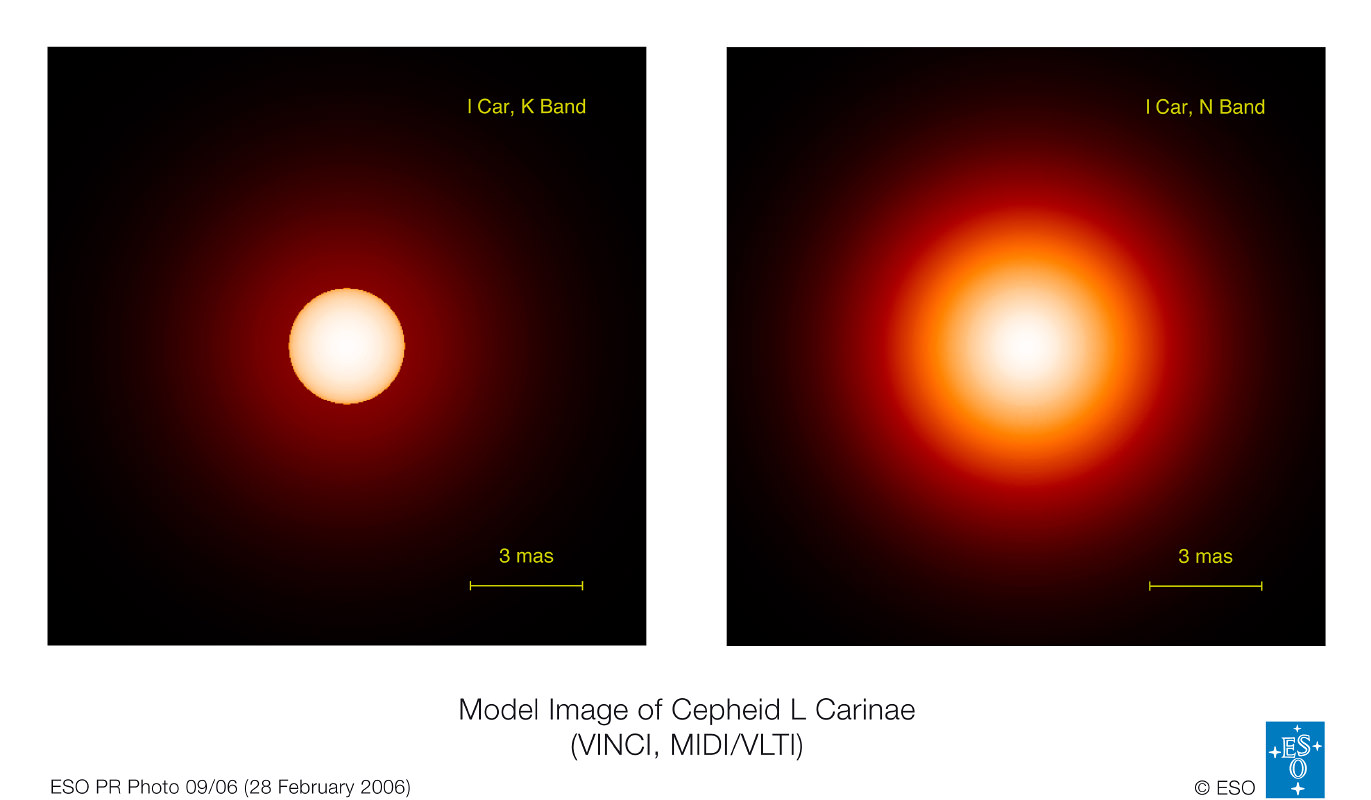
\includegraphics[width=\textwidth]{cepheid.png}
        \end{center}
    \column{.5\textwidth}
        \begin{center}
             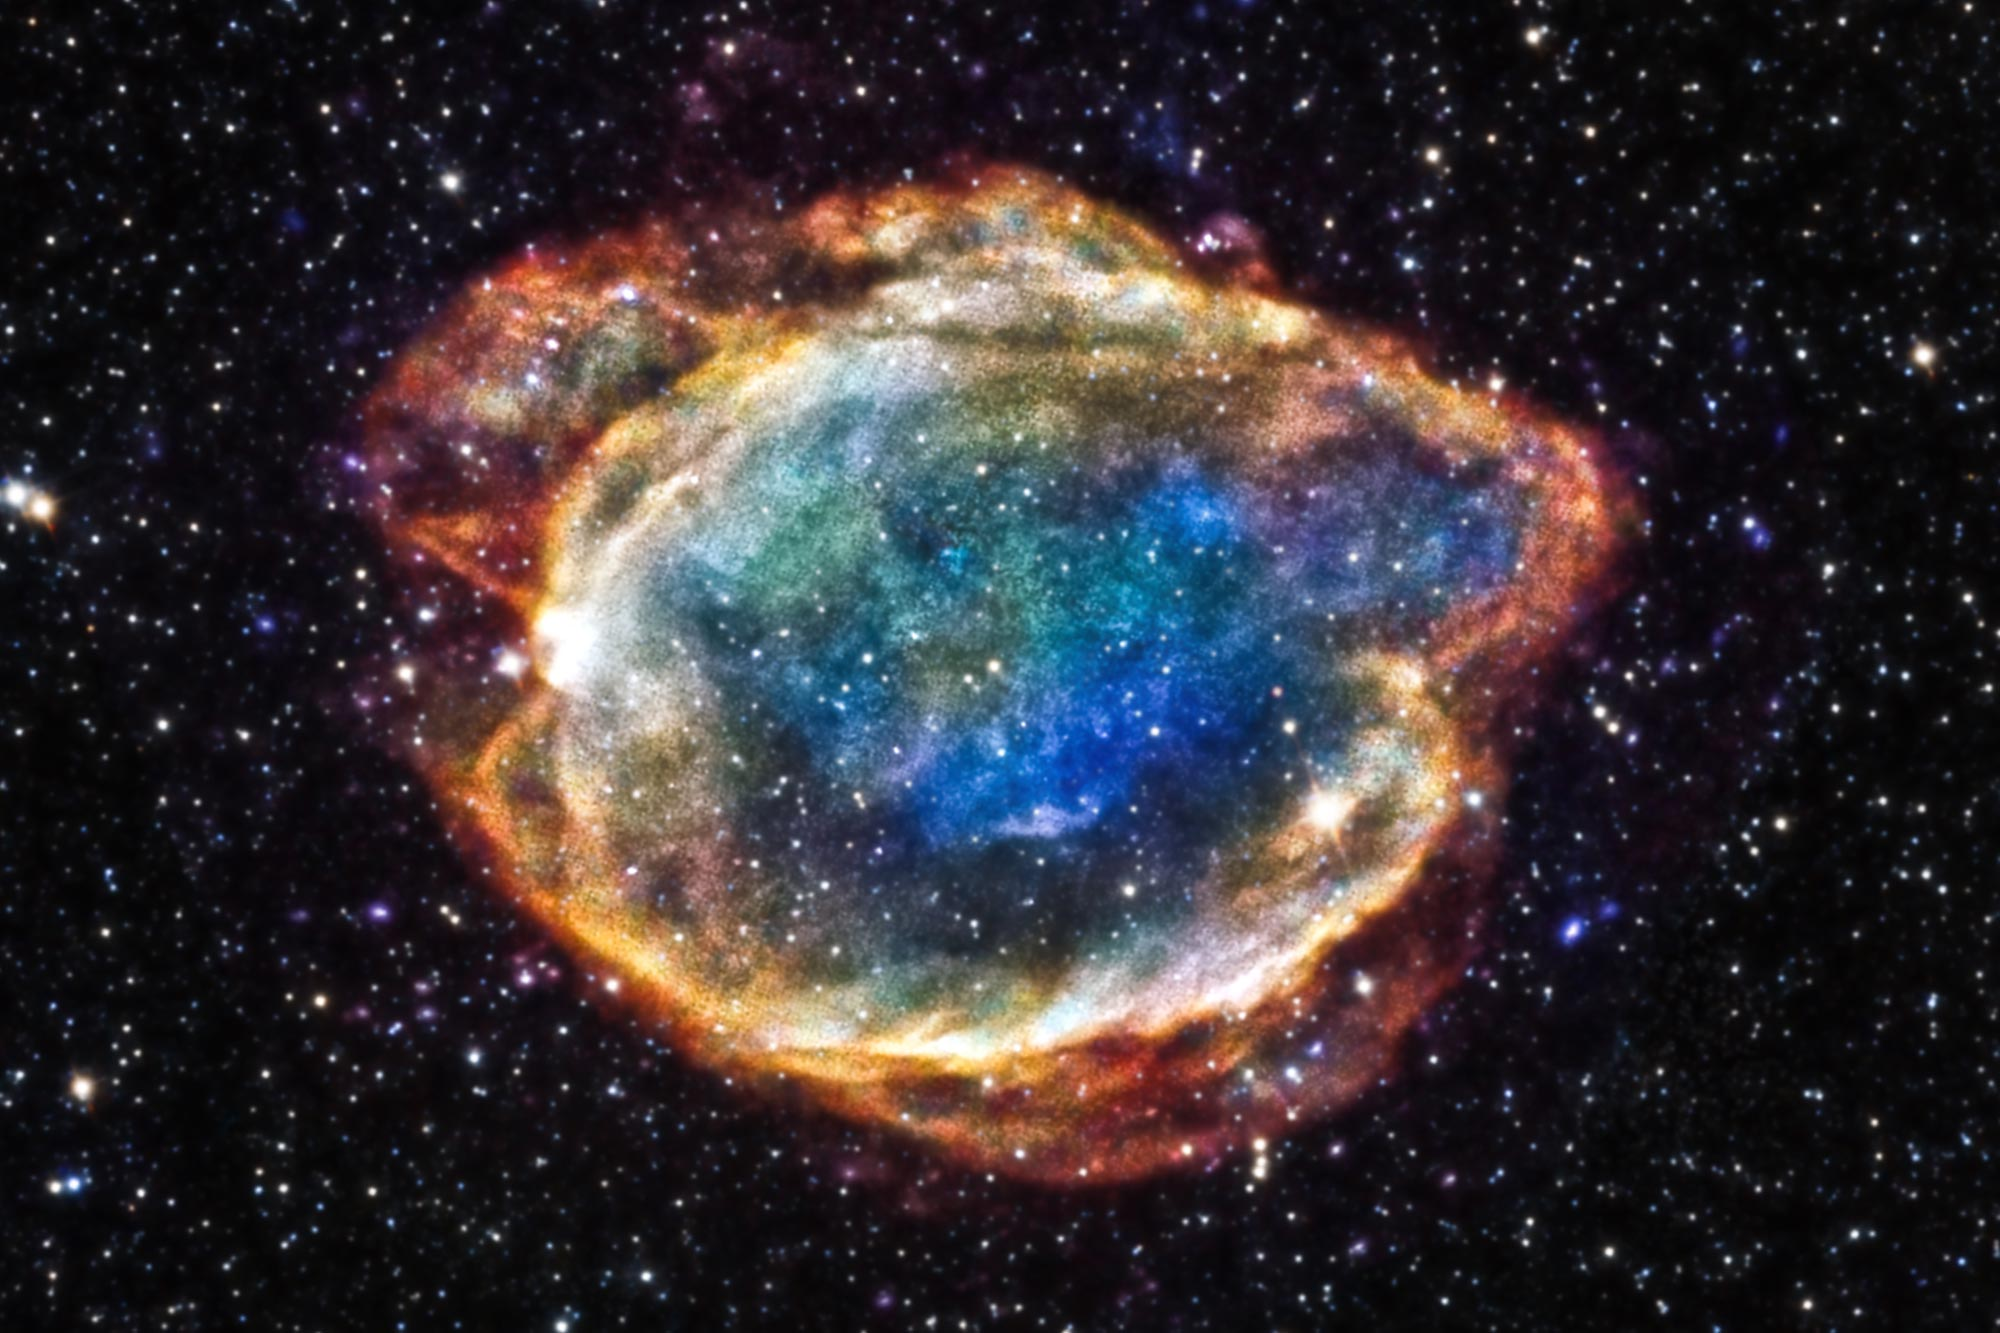
\includegraphics[width=\textwidth]{supernova.png}
        \end{center}
\end{columns}

\end{frame}

\begin{frame}
	It was observed that the luminosity observed by a human eye is in
	logarithmic scale, which also has a historical significance of Greeks
	dividing stars into different apparent brightness scales.

	\begin{enumerate}
		\item Thus the
			\textbf{apparent magnitude} of a light source is defined in terms of the source's
	bolometric flux
	$$ m = -2.5 \log_{10}(f/f_x) $$

\item Similarly we define \textbf{absolute magnitude} of a light source is
	defined wrt. to the apparent magnitude when its distance $d_L = 10 pc$
	$$ M = -2.5 \log_{10}(L/L_x) $$

	Thus we can find luminosity distance using these metrics as:
	$$ m - M = 5 log_{10} \left( \frac{d_L}{1 Mpc} \right) + 25$$

        \end{enumerate}
\end{frame}


% Ending page
\section*{Was it Fun?}
\begin{frame}{Was it Fun?}

Yes, ryden has a very creative of explaining things, and gives enough time to appreciate
historical aspects too, and always includes metaphors and poems.

\begin{columns}[c]
    \column{.5\textwidth}
        \begin{center}
            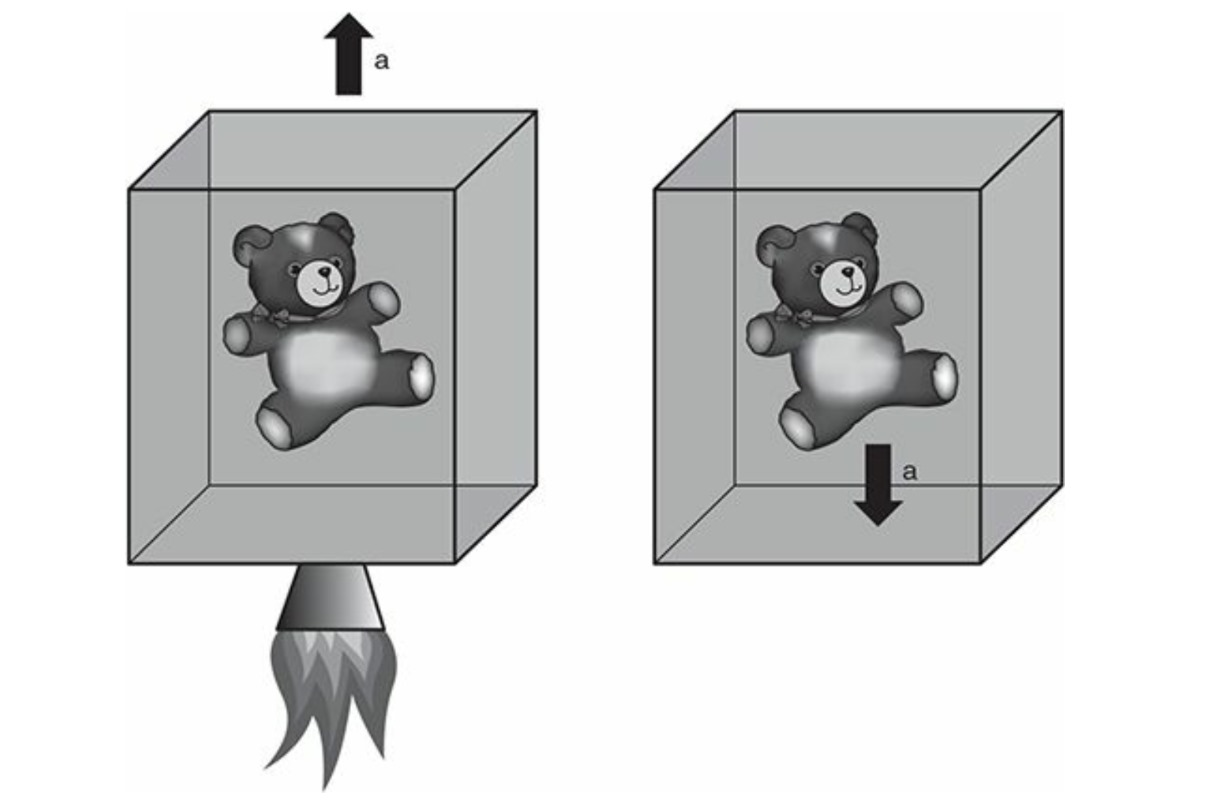
\includegraphics[width=\textwidth]{teddy}
        \end{center}
    \column{.5\textwidth}
        \begin{center}
             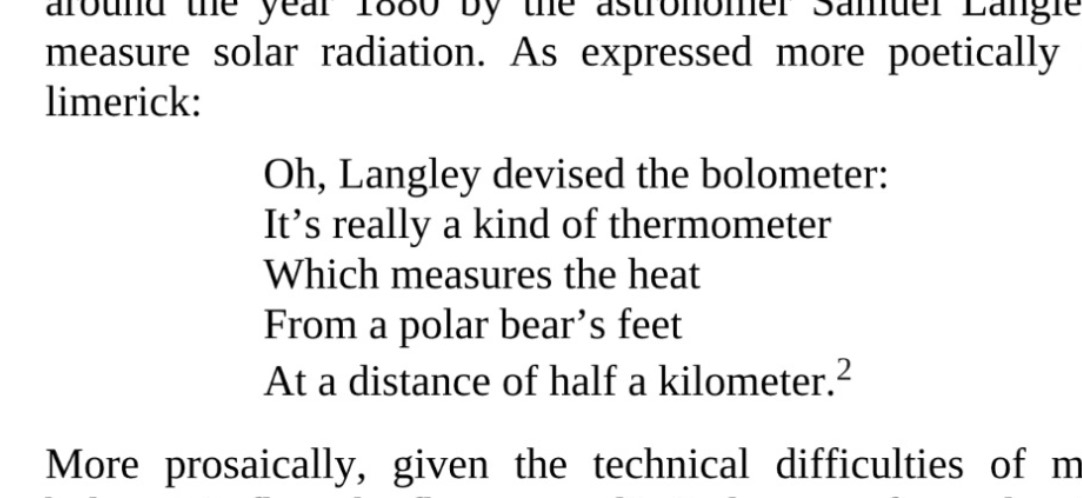
\includegraphics[width=\textwidth]{destiny}
        \end{center}
\end{columns}

\end{frame}

\begin{frame}
  \begin{beamercolorbox}[sep=8pt,center,shadow=false,rounded=true]{title}
  \centering \Huge
  Thank You
  \end{beamercolorbox}
\end{frame}

\end{document}
